\documentclass{article}
\usepackage[frenchb]{babel}
\usepackage{amsfonts}
\usepackage{amsmath}
\usepackage[T1]{fontenc}
\usepackage[utf8]{inputenc}
\usepackage{amsthm}
\usepackage{graphicx}
\usepackage{tikz-cd}

\title{Méthodes ABC en épidémiologie}
\author{ Cl\'ement Dell'Aiera}
\date{}

\theoremstyle{definition}
\newtheorem{definition}{Definition}
\newtheorem{thm}{Théorème}
\newtheorem{ex}{Exercice}
\newtheorem{lem}{Lemme}
\newtheorem{dem}{Preuve}
\newtheorem{prop}{Proposition}
\newtheorem{cor}{Corollaire}

\newcommand{\Z}{\mathbb Z}
\newcommand{\Q}{\mathbb Q}
\newcommand{\R}{\mathbb R}
\newcommand{\C}{\mathbb C}
\newcommand{\Hil}{\mathcal H}
\newcommand{\Mn}{\mathcal M _n (\mathbb C)}
\newcommand{\K}{\mathbb K}
\newcommand{\B}{\mathbb B}
\newcommand{\Cat}{\mathbb B / \mathbb K}

\begin{document}
\maketitle

\begin{abstract}

\end{abstract}


\newpage
\tableofcontents

\newpage

\setlength{\parindent}{0cm}

\section{Principe et historique}

\subsection{Méthodes ABC.}

%Les méthodes de l'inférence bayésienne se basent sur le calcul de la vraisemblance du modèle.
Rappelons le principe de l'inférence bayésienne : le modélisateur se donne un prior $\pi$ sur le paramètre $\theta$ et une famille de loi $p(x|\theta)$. Suite à des observations $x$, on met à jour la loi, i.e. on cherche à calculer :
\[p(\theta|x)=\frac{p(x|\theta)\pi(\theta)}{p(x)})\]
où: $p(x)=\int p(x|\theta)\pi(\theta) d\theta$. Cette dernière intégrale peut être difficile à calculer numériquement, typiquement si l'espace des paramètre $\Theta$ est de grande dimension, mais cette difficulté peut être traitée avec des algorithmes classiques tels que Monte Carlo Markov Chains par exemple, où les modélisateur a seulement besoin de connaître la loi a posteriori à une constante de normalisation près, pour pouvoir simuler des paramètres selon des données observées.\\

Ces méthodes que nous avons appelées "classiques" comportent néanmoins un inconvénient majeur : l'expérimentateur n'a aucun contrôle sur l'erreur commise dans l'approximation de sa loi $p$ par des $X_n$ , i.e. l'entier :
\[N_\epsilon = \inf_{n}\{\forall m\geq n,|P(X_m=\theta)-p(x)|<\epsilon\}\]
est bien défini, mais n'est pas calculable de façon universelle. \\

Toutefois si la loi est discrète et de basse dimension, Rubin a proposé un algorithme qui permet de simuler des paramètres à partir de données sans vraisemblance.\\

\fbox{\begin{minipage}{0.9\textwidth}
  Soit $y$ une observation, tant que le nombre de simulations acceptées est inférieur à $N$, répéter :
\begin{enumerate}
\item Simuler $\theta_i \sim \pi(\theta)$
\item Simuler $x_j \sim p(x|\theta)$
\item Si $x_j\neq y$, rejeter $x_j$.
\end{enumerate}
\end{minipage}}\\
\\

On voit que si les données suivent une loi continue, la probabilité que l'algorithme accepte un nombre non nul de simulation est $0$. Rubin a alors proposé une modification de l'étape 3 basé sur une discrépance $\rho$ qui fait office de distance entre les observations et les points simulés. Pour illustrer par un exemple simple, on peut imaginer que $\rho$ est la distance euclidienne usuelle.\\
\\

\fbox{\begin{minipage}{0.9\textwidth}
  Soit $y$ une observation, tant que le nombre de simulations acceptées est inférieur à $N$, répéter :
\begin{enumerate}
\item Simuler $\theta_i \sim \pi(\theta)$
\item Simuler $x_j \sim p(x|\theta)$
\item Si $\rho(x_j,y)>\epsilon$, rejeter $x_j$.
\end{enumerate}
\end{minipage}}
\\
\\

Pour s'attaquer aux grandes dimensions, on peut se servir d'une application $S$ à valeur dans un espace de petite dimension et aboutir à une autre version de ce même algorithme. On impoose à $S$ de vérifier : $p(\theta|x)=p(\theta|S(x)),\forall \pi$ afin de limiter la perte d'information : cette application $S$ peut être pensée comme une statistique exhaustive pour le modèle.
\\

\fbox{\begin{minipage}{0.9\textwidth}
  Soit $y$ une observation, tant que le nombre de simulations acceptées est inférieur à $N$, répéter :
\begin{enumerate}
\item Simuler $\theta_i \sim \pi(\theta)$
\item Simuler $x_j \sim p(x|\theta)$
\item Si $\rho(S(x_j),S(y))>\epsilon$, rejeter $x_j$.
\end{enumerate}
\end{minipage}}
\\
\\

Pour résumer, la méthode ABC (Approximate Bayesian Computing) propose, si l'on veut estimer la distribution \textit{a posteriori} d'un paramètre $\theta$, de simuler des variables $\theta_j$ selon notre \textit{prior} $\pi$, à partir desquelles sont simulées des échantillons $y_j$, $j$ allant de $1$ à $n$ le nombre de simulations. Un ensemble de \textit{summary} $S(y_j)$ est alors calculé à partir des données simulées, quantités que l'on compare à la valeur $S(y_0)$ de $S$ sur le véritable échantillon observé. Si la "distance" entre $S(y_j)$ et $S(y_0)$ ne dépasse pas un certain seuil $\epsilon$ fixé à l'avance, on garde la simulation $\theta_j$, sinon on la rejette.  

\subsection{Un exemple simple}

Nous allons illustrer le dernier algorithme sur un exemple simple. On se place dans le cas d'un modèle bayésien avec un prior normal $\pi(\theta)\sim \mathcal N(0,1)$ et d'une loi $p(x|\theta)\sim\mathcal N(\theta,1)$. On sait que les lois normales sont conjuguées :
\[p(\theta|x)\sim\mathcal N (x,\frac{1}{2}).\]
Regardons ce que Scilab nous donne à partir de l'observation $x=1$, de $5000$ simulations (acceptées) et de $\epsilon=0.01$.

\begin{figure}[h]\centering
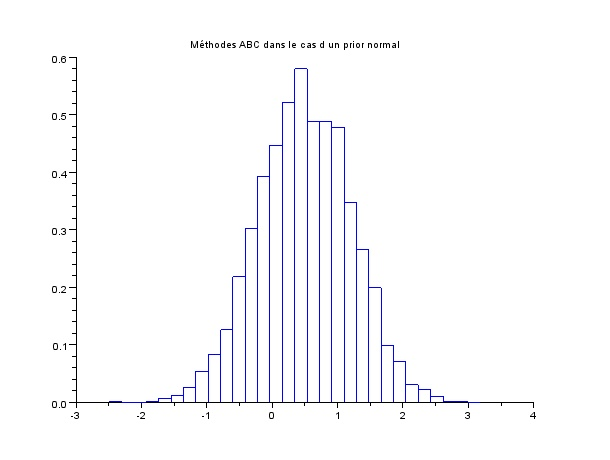
\includegraphics[scale=0.6]{ABCnorm.jpg}
\caption{Histogramme de 5000 simulations de $\theta$}
\label{fig:ABCnorm}
\end{figure}

\section{Trois algorithmes importants en méthode ABC}

\subsection{Correction par régression locale}
 Nous l'avons vu, la méthode ABC ne permet pas de simuler exactement la loi désirée. La méthode de correction par régression locale propose de corriger cet écart en utilisant le modèle de régression :
\[\theta_i=f(S(x_i))+\epsilon_i\]
où $f$ est la fonction de régression et les $\epsilon_i$ sont centrés de même variance. On note $y$ la valeur observée. Le principe est le suivant : on donne un poids plus fort aux simulations qui sont le plus proches de $S(y)$. Pour cela, à chaque simulation $(\theta_i,S(x_i))$ est associé le poids :
\[K(\rho(S(x_i),S(y))\] 
où l'on s'est fixé le noyau $K$ à l'avance. Une fois la régression effecuée, on obtient un échantillon pondéré de la loi \textit{a posteriori} en corrigeant les $\theta_i$ comme suit,
\[\theta^*_i=\hat f(S(y))+\frac{\hat\sigma(S(y))}{\hat\sigma(S(x_i))}\hat\epsilon_i\]
où $\hat f$ est l'ésperance conditionnelle estimée, les $\hat\epsilon_i$ sont les résidus empiriques de la régression, et $\hat\sigma$ dénote l'écart-type empirique conditionnel.\\

Il est possible d'utiliser un réseau de neurone à la place de la régression. Nous proposerons d'utiliser ces deux méthodes dans la partie$2$ sur des exemples, grâce au package \textbf{abc} du logiciel $R$. Voici un algorithme qui se base sur cette méthode, issu de l'article de Beaumont.
\\

\fbox{\begin{minipage}{0.9\textwidth}
\begin{enumerate}
\item Si $y$ est une observation, tant que le nombre de simulations est inférieur à $M$:
	\begin{enumerate}
	\item Simuler $\theta_i \sim \pi(\theta)$
	\item Simuler $x_i \sim p(x|\theta_i)$
	\end{enumerate}
\item Soit $k_j\leftarrow $ l'écart type empirique des $S_j(x)$
\item $\rho(S(x),S(y)):= \sqrt{\sum_{j=1}^s (S_j(x)-S_j(y))^2}$
\item Choisir la tolérance $\epsilon$ telle que la proportion de points acceptés $P_\epsilon$ vaille $N/M$
\item Pondérer les simulations $S(x_i)$ avec $K_\epsilon(\rho(S(x_i),S(y)))$,  où \[K_\epsilon(t)=\epsilon^{-1}(1-(t/\epsilon)^2)1_{t\leq \epsilon}(t)\]
\item Estimer $\hat E [\theta|S(x)]$ grâce à une régression linéaire pondérée appliquée aux $N$ points de poids non nuls
\item Ajuster $\theta^*_i=\theta_i-\hat E [\theta|S(x_i)]+\hat E [\theta|S(y)]$
\item Les $\theta_i^*$ obtenus, de poids $K_\epsilon(\rho(S(x_i),S(y)))$, sont des simulations approchées de la loi \textit{a posteriori} $p(\theta|y)$
\end{enumerate}
\end{minipage}}\\
\\

\subsection{Algorithme MCMC dans le cadre ABC}

Dans cette section, on détaille l'algorithme MCMC adapté au cadre ABC. Un inconvenient des méthodes par rejet et régression ABC (que nous illustrerons dans la partie 2) est que l'on simule les paramètres selon le \textit{prior} sans tenir compte de l'information qu'apporte l'échantillon. Typiquement, un échantillon qui apporterait beaucoup d'information permet, en concentrant la loi \textit{a posteriori}, de simuler des paramètres de façon plus efficace selon cette dernière. Toutefois, le calcul de la loi \textit{a posteriori} peut être très difficile en pratique, d'où l'idée d'utiliser les méthodes de Monte Carlo Markov Chain, que nous avons rappelées précédement. Nous suivons l'article de Beaumont pour présenter une algorithme MCMC adapté aux méthodes ABC. \\

On commence par simuler selon le \textit{prior} $\pi(\theta)$, ce qui nous donne notre état initial. Pour passer d'un état à un autre, on utilise une loi que l'on choisit par exemple un noyau gaussien, que l'on note $K$. Ce noyau nous propose un éventuel nouvel état, que l'on accepte ou pas en fonction d'une valeur seuil.\\ 
\\

\fbox{\begin{minipage}{0.9\textwidth}
 Initialisation : Simuler $\theta_0 \sim\pi(\theta)$.\\
Pour $n$ allant de $1$ au nombre de simulations souhaité, faire : 
\begin{enumerate}
\item Simuler $\theta' \sim K(\theta|\theta_{n-1})$
\item Simuler $x \sim p(x|\theta')$
\item Si $\rho(S(x)S(y))<\epsilon$,
	\begin{enumerate}
	\item Simuler $u\sim \mathcal U_{[0;1]}$
	\item Si  $u\leq \pi(\theta')/\pi(\theta_{n-1}) \times K(\theta_{n-1}|\theta')/K(\theta'|\theta_{n-1})$\\
		$\theta_n=\theta'$;
	\item Sinon $\theta_n=\theta_{n-1}$ 
\end{enumerate}
\item Sinon $\theta_n=\theta_{n-1}$
\end{enumerate}
\end{minipage}}\\
\\

Cette méthode présente un inconvénient : le taux d'acceptation des états peut être très faible. Il est en effet proportionnel à la fréquence à laquelle les paramètres tels que $\rho(S(x),S(y))<\epsilon$ sont simulés, ce qui diffère des méthodes MCMC classiques, où le taux d'acceptation est proportionnel au rapport des deux vraisemblances entre état proposé et état courant. Beaumont fait remarquer dans son article qu'un mauvais choix de l'état initial par exemple loi dans la queue de la distribution de $\pi(\theta)$, peut conduire à des taux très bas, ce qui ralentit fortement les méthodes.\\

\subsection{Méthodes de Monte-Carlo Séquentielles}

Les méthodes SMC (Sequential Monte Carlo) permettent d'estimer des variables cachées $x_i$ en observant seulement des $y_j$, en supposant que $x$ soit une chaîne de Markov et que les $y_j|x$ soient indépendants. Un exemple immédiat est celui du filtre de Kalman, ou plus généralement si :
\[\left\{ \begin{array}{l} x_{n+1}=f(x_n)+\epsilon_n \\ y_n=g(x_n)+\eta_n\end{array} \right.\]
où les suites $\epsilon$ et $\eta$ sont par exemple des bruits blancs indépendants. On suppose que l'on connaît $f$,$g$, ainsi que la distribution de $\epsilon$ et $\eta$. \\

Voici un algorithme SMC adapté au cadre ABC proposé dans l'article de Beaumont :\\

\fbox{\begin{minipage}{0.9\textwidth}
On se donne une suite décroissante de seuils : $\epsilon_1..\epsilon_T$\\
Pour $n$ allant de $1$ au nombre de simulations souhaité $N$, faire : 
\begin{enumerate}
\item A l'instant $t=1$,\\
	Pour $i=1,..,N$,\\
	Tant que $\rho(S(x),S(y))<\epsilon_1$\\
	Simuler $\theta_i^{(1)}\sim\pi(\theta)$ et $x\sim p(x|\theta_i^{(1)})$\\
	$w_i\leftarrow1/N$\\
	$\tau^2_2\leftarrow 2 \times \big($ variance empirique des $\theta_i^{(1)}\big)$
\item A l'instant $t, \quad 2\leq t \leq T$\\
	Pour $i=1,..,N$,\\
	Tant que $\rho(S(x),S(y))<\epsilon_t$\\
	Tirer aléatoirement $\theta_i^*$ des $\theta_j^{(t-1)}$, chacun affecté de la probabilité $w_j^{(t-1)}$\\
	Simuler $\theta_i^{(t)}\sim K(\theta|\theta^*_i;\tau_t^2)$ et $x\sim p(x|\theta_i^{(t)})$\\
	Choisir les poids $w_i \propto \pi(\theta_i^{(t)}/\sum_j=1^N w_j^{(t-1)} K(\theta_i^{(t)}|\theta^{(t-1)}_j;\tau_t^2)$\\
	$\tau^2_{t+1}\leftarrow 2 \times \big($ variance empirique pondérées des $\theta_i^{(t)}\big)$
\end{enumerate}
\end{minipage}}\\
\\

\section{Application en épidémiologie}

\subsection{Modèle SIR avec contact tracing}

Nous étudierons dans cette partie l'application des méthodes ABC à l'épidémie du VIH à Cuba suivant l'article de Blum et Tran ~\cite{BlumTran}. Le modèle est formé de trois variables : les individus sains $S$, les individus infectés $I$, et les individus repérés $R$. On suppose qu'une fois un individu repéré, il ne contamine plus personne, et est soit dans la classe $R_1$ s'il a été repéré par un test aléatoire (prise de sang, grossesse,...), soit dans la classe $R_2$ s'il l'a été par contact tracing. On peut quitter où arriver dans une certaines classe au taux indiqués dans la figure \ref{SIR}.\\
\begin{figure}[!h]\centering
\begin{tikzcd}
	{}	&		{}	&					{}		&  R_1\\
 \arrow{r}{\lambda_0} &   S \arrow{r}{\lambda_1 SI} \arrow{d}{\mu_0 S} &  I \arrow{d}{\mu_1 I}\arrow{ru}{\lambda_2 I}\arrow{rd}{\lambda_3 \sum e^{-c(T-T_i)}} & {}\\
              {}  &               {}                   &  		{}		& R_2\\
\end{tikzcd}
\caption{Modèle SIR incorporant le contact-tracing.}
\label{SIR}
\end{figure}

On notera $\theta=(\mu_1,\lambda_1,\lambda_2,\lambda_3,c)$, qui paramètre le modèle. Il a été démontré par Clemençon \textit{et al.}~\cite{Clemencon} que le système d'EDS obtenu à partir de ce modèle converge à la limite macroscopique (population de grade taille) vers les équations classiques de l'épidémiologie :
\[\left\{\begin{array}{rl} s'_t& = \mu_0-\lambda_0 s_t -\lambda_1 s_t i_t \\
                       i'_t  & =\lambda_1 s_t i_t -(\mu_1+\lambda_2)i_t -\lambda_3i_t\int \varphi (a) \rho_t(a) da \\
		\rho_t(0) &= \lambda_2 i_t +\lambda_3 i_t \int \varphi (a) \rho_t(a) da  \\
\end{array}\right.\]
(ici $\varphi(t)=e^{-ct}$)\\

Voici un algortihme de simulation du modèle tiré de ~\cite{BlumTran}:\\

\fbox{\begin{minipage}{0.9\textwidth}
\begin{enumerate}
\item Initialisation : $S=S_0$ individus sains, $I=I_0$ individus infectés, $R_i=0$ individu détécté. Temps d'arrêt $T>0$.\\
Sachant que l'on a simulé $k$ événements aus temps $t_j$ pour $j=1,k$, et que le temps courant $\tau = t_k$ :
\item Simuler une exponentielle $\mathcal E (C_k)$ où \[C_k = \lambda_1 S_{t_k} I_{t_k}+(\mu_1+\lambda_2) I_{t_k}+\lambda_3 I_{t_k} R_{t_k}.\]
\item Actualiser le temps courant $\tau \leftarrow \tau +\mathcal E$.
\item Si $\tau > T$, fin. Sinon : simuler une uniforme $U$ sur $[0,C_k]$ et 
\begin{enumerate}
\item Si $0 \leq U \leq  \lambda_1S_{t_k} I_{t_k}$ : $S \leftarrow S-1$ et $I \leftarrow I+1$ .
\item Si $\lambda_1 S_{t_k} I_{t_k} \leq U \leq  \lambda_1 S_{t_k} I_{t_k}+\mu_1 I_{t_k}$ : $I \leftarrow I-1$ .
\item Si $\lambda_1 S_{t_k} I_{t_k}+\mu_1  I_{t_k} \leq U \leq  \lambda_1 S_{t_k} I_{t_k}+(\mu_1+\lambda_2) I_{t_k}$ : $I \leftarrow I-1$ et $R_1 \leftarrow R_1+1$ . 
\item Si $\lambda_1 S_{t_k} I_{t_k}+(\mu_1+\lambda_2) I_{t_k} \leq U \leq \lambda_1 S_{t_k} I_{t_k}+(\mu_1+\lambda_2) I_{t_k} +\lambda_3 I_{t_k} \sum e^{-c(\tau-T_i)}$ : $I \leftarrow I-1$ , $R_2 \leftarrow R_2+1$ 
\item Sinon : ne rien faire.
\end{enumerate} 
\end{enumerate}

\end{minipage}}\\
\\

\newpage

\bibliographystyle{plain}
\bibliography{biblio} 
\nocite{*}
\end{document}

























